\documentclass[11pt]{article}         

%SJ: Packages we added
\usepackage{geometry}
\geometry{letterpaper}
\usepackage{graphicx}
\usepackage{amssymb,amsfonts,amsmath}
\usepackage{epstopdf}
\DeclareGraphicsRule{.tif}{png}{.png}{`convert #1 `dirname #1`/`basename #1 .tif`.png}
\usepackage[footnotesize]{caption}
\usepackage{capt-of}

\usepackage{booktabs}
\usepackage{amsmath}
\usepackage{color}
\usepackage[normalem]{ulem} %This allows for strikethrough.  The corresponding command in text is 
	% \sout{<text>}
	
%Steph added:
\usepackage[usenames,dvipsnames]{xcolor}
\newcommand{\sj}[1]{\textcolor{red}{#1}}

\bibliographystyle{unsrt}

\oddsidemargin -0.1in
\evensidemargin -0.1in
\textwidth 6.75in
\headheight 0.0in
\topmargin -0.5in
\textheight=8.7in

\begin{document}

\title{Analysis code for smFRET: Documentation}

\author{%
Stephanie Johnson,\\Department of Biochemistry and
     Biophysics, \\University of California, San Francisco, \\San Francisco, CA, USA\\
%\and Matthew Johnson,\\Department of Electrical Engineering and Computer Science, \\Massachusetts Institute of
%    Technology, \\Cambridge, MA, USA\\
%\and Luke Breuer\\San Francisco, CA, USA
}
\date{}

\maketitle

\tableofcontents

\newpage

\section{Introduction.}

This is a software suite designed to calculate FRET-versus-time traces from a standard prism TIRF-based single-molecule FRET microscopy setup.  The most current version of this suite can be found at $<$https://github.com/stephlj/smFRETcode$>$.  It can be run as a stand-alone analysis suite, but it is written as modularly as possible in the hopes that it can be adapted fairly easily for other microscopy setups and acquisition software.  A limited number of setup-specific parameters can be changed in the smFRETsetup file, but it is likely that you will need to modify at least some parts of this code (for example, the file loading function, unless images from your camera are saved the same way ours are---see more details below). %Section~\ref{sec:CustomOpts} below discusses some additional options for customizing this suite to suit your particular needs.

The general outline of the analysis workflow is: (1) Calculate a map that correlates pixels in the acceptor channel image to pixels in the donor channel image, as these will never be perfectly aligned in an smFRET setup. Or, load an old one. (2) Find fluorescent spots in a movie or set of movies and allow the user to scroll through intensity-versus-time traces for each spot, and then save good traces for further analysis later.

The rest of this manual contains information about required Matlab toolboxes, a walkthrough of how to run an analysis session off-the-shelf, and details of how the analysis is done.

%For getting started, sample data (of double-stranded DNAs with a Cy5 on one end and and internally labeled Cy3 5~bp away) can be downloaded from https://github.com/stephlj/smFRETdata \sj{(TODO upload sample data)}. 

\subsection{Licensing and copyright information.}

Software and manual copyright \copyright 2014 Stephanie Johnson, University of California, San Francisco.

This program is free software: you can redistribute it and/or modify
    it under the terms of the GNU General Public License as published by
    the Free Software Foundation, either version 3 of the License, or
    (at your option) any later version.

    This program is distributed in the hope that it will be useful,
    but WITHOUT ANY WARRANTY; without even the implied warranty of
    MERCHANTABILITY or FITNESS FOR A PARTICULAR PURPOSE.  See the
    GNU General Public License for more details.

    A copy of the GNU General Public License can be found in the LICENSE.txt file that accompanies this software; it can also be found at $<$http://www.gnu.org/licenses/$>$.
    
\subsection{Contact information.}

If you have questions or comments about this software suite, please open an issue through the github repository for this suite (preferred), or contact me at Stephanie.Johnson@ucsf.edu (most recent contact information can be found on my github account).  If you find a bug in this code, I would love to hear about it.  Please include as much information as you can about what causes the bug---what commands you entered, a screen shot of the output, etc, and even some of your data, if you can.  Thanks!

\clearpage

\section{Getting started.}

\subsection{General requirements.}

Requires Matlab with the following toolbox installed:\\

\noindent \textbullet~Image Processing Toolbox\\

\noindent and will use the following if available:\\

\noindent \textbullet~Curve Fitting Toolbox

\noindent \textbullet~Optimization Toolbox\\

\noindent This code was written for analyzing prism-based TIRF images; it may not work as well for objective-based setups (for example, you may have to alter or re-write the code to find spots, or do a more sophisticated background subtraction).\\

\noindent The background subtraction (see Sec.~\ref{sec:BkgndSub}) creates a set of additional files that get saved to the same directory as the raw image file(s) to be analyzed, and could be as large as 4 times the original movie size.  Meaning, if you take a 1 GB movie, whatever drive you load this 1 GB movie from needs to have at least 4 GB of free space! 

\subsection{Data format requirements.}

This software assumes the following about how raw data area acquired and stored from the camera:\\

\noindent \textbullet~We acquire data with the open-source UCSF software Micro-Manager (http://www.micro-manager.org/), using its Multi-D acquisition tool. Micro-Manager stores the raw data as .tif files, in directories entitled \textit{rootname\_1, rootname\_2, etc}, where ``rootname'' is defined by the user prior to acquisition, and a new folder with \_1, \_2 etc is created for each acquisition with the same rootname.  Each of the resulting directories contains one tiff per frame from the acquired movie (if the ``save as separate image files'' option is selected in Micro-Manager), with filenames img\_000000000\_000.tif, img\_000000001\_000.tif, etc. In each movie's directory Micro-Manager also saves a metadata.txt file with information about frame rate, etc.  This suite analyzes everything with the same rootname in one batch and saves the analysis to one final directory, also called rootname.  More specifically, all directories called \textit{rootname*}, where * is a wildcard and represents any number of any character(s), will be analyzed together and the results saved to one final directory. \\

\noindent \textbullet~The function LoadUManagerTifs, called by LoadRawImgs, assumes data images are stored as ``img*.tif'', with one tiff per frame.\\

\noindent \textbullet~The function LoadRawImgs assumes the file and directory structure created by Micro-Manager (summarized in Fig.~\ref{fig:DirectoryStructure}); if you use something other than Micro-Manager to acquire data, and want to use this suite out-of-the-box, you will have to reorganize your data into the directory structure that LoadRawImgs and smFRET recognize.  Alternatively, you can modify LoadRawImgs and its dependences (see Figs.~\ref{fig:CodeConnectivity1} and~\ref{fig:CodeConnectivity2} below), and some sections of the main smFRET function, to recognize your data structure (those are probably the only two sets of functions you'll have to modify).  \\

\noindent \textbullet~This suite is also capable of loading the .pma binary files saved by the Ha lab acquisition software (and used by their IDL analysis software), instead of tiffs.  Type ``help LoadPMA'' in the command line in Matlab for more information about the assumed structure of these .pma files.  However, the directory structure created by Micro-Manager is still assumed---that is, you should put each .pma file in its own directory, and, if you want to analyze multiple pma's in one batch, call each directory \textit{rootname\_1, rootname\_2, etc} with each of these directories having one and only one pma.  The filename of the pma's can be whatever you want, but there can only be one per directory. (Or you can call the directories \textit{rootnameA, rootnameB, etc}---just so long as they're a sequence of \textit{rootname*}.) NOTE: if both a pma and a tiff(s) exist in the same folder, it will default to using the pma! \\

\noindent \textbullet~Additionally, if your acquisition software does not save a metadata.txt file, you will have to create one yourself, or modify GetInfoFromMetaData.m; type ``help GetInfoFromMetaData'' for information about how to create your own.  A sample metadata.txt file is also included with this software.  Each directory to be analyzed must have a metadata.txt.\\ 


\begin{figure}[!t]
\begin{center}
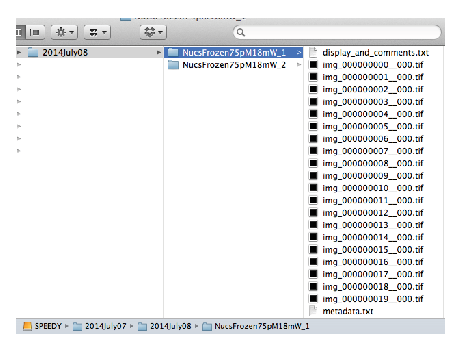
\includegraphics[width=4.5in]{ScreenShots/DirectoriesShot.eps}
\caption{Screen shot illustrating the directory structure assumed by smFRET.m and LoadRawImgs.m.  Here ``rootname'' is ``NucsFrozen75pM18mW''; so to analyze both of these subfolders together, the call to smFRET would be smFRET(`NucsFrozen75pM18mW').  If your acquisition software creates pma's rather than tif's, the ``NucsFrozen75pM18mW\_1'' directory would have one .pma file instead of all of the .tif files, and a metadata.txt file, but not the display\_and\_comments.txt file (a file saved by Micro-Manager that we don't use).  You don't need to have multiple directories that you want to analyze at once. The highlighted directory in the middle column containing images to be analyzed will be called ``datadir'' in the rest of this manual.}
\label{fig:DirectoryStructure}
\end{center}
\end{figure}

\noindent \textbullet~Channel mapping (at least an initial one) is accomplished by means of images of fluorescent beads that are visible in both channels. It is assumed these beads are in directories that contain the word ``Bead'' ({\it e.g.}, ``Beads\_1'', ``Beads\_2''). Although it is not assumed there are movies (rather than single frames) in these directories, I've found it's better to average 10-20 frames before finding bead positions.  It is possible to skip the channel mapping with beads step, but your channels will have to start out fairly well aligned (see also below where the details of the channel mapping process are discussed).\\

\noindent \textbullet~While you can set certain setup-specific parameters in smFRETsetup.m, such as whether the donor channel is the right half or left half (or top or bottom) of the image, you will have to write your own wrapper function for certain extensions such as images obtained on a three-color FRET setup.

\subsection{Overview of the analysis process.}

The workflow for analyzing smFRET data is, generally speaking, composed of five steps (which I will refer to as ``modules''): (1) data pre-processing (which includes things like scaling each image to take advantage of the full dynamic range of the numeric type you're using); (2) finding a mapping between the donor and acceptor channels (which will never be perfectly aligned in any setup, so that a mathematical relationship between points in one channel to points in the other must be calculated, in order to identify FRET pairs); (3) spot finding (identifying which pixels contain fluorescence from real molecules, and which are background fluctuations); (4) calculating the intensity in each identified spot in each frame, and from these intensities, FRET-versus-time traces; and finally (5) displaying these traces for the user to comb through to pick out real results for further analysis.  I have found that thinking about the analysis workflow in terms of these five modules has been helpful, but note that modules are not necessarily performed in the order listed above; for example, we do a channel mapping (module 2) before data pre-processing (module 1), and this analysis suite also offers the opportunity to make a refined map (module 2) using FRET pairs that the user has looked through (module 5).

Details of how to run each module, and of what each module does to the data, are discussed in the next section.  Figures~\ref{fig:CodeConnectivity1} and~\ref{fig:CodeConnectivity2} show call graphs that diagram the functions in this analysis suite that perform each module, with any required or optional Matlab toolboxes noted to the right of each function. Functions in colored boxes are ``tools'' that are called by multiple functions; pink are highly specific to our microscope setup, yellow should be more general.  Blue asterisks indicate interactive sections requiring user input; red arrows indicate files saved to or loaded from disk (dashed lines indicate optional pathways based on user input).

There is one function that is included in this suite but not listed in Figs~\ref{fig:CodeConnectivity1} and~\ref{fig:CodeConnectivity2}, because it is not called by smFRET directly.  This function is ``ConvertTovbFRETInput.m'' and converts any saved traces (see Sec.~\ref{sec:GUI} below) to an input format recognized by the vbFRET analysis software for doing hidden Markov analyses of FRET data \cite{Bronson2009}.

\begin{figure}[!p]
\begin{center}
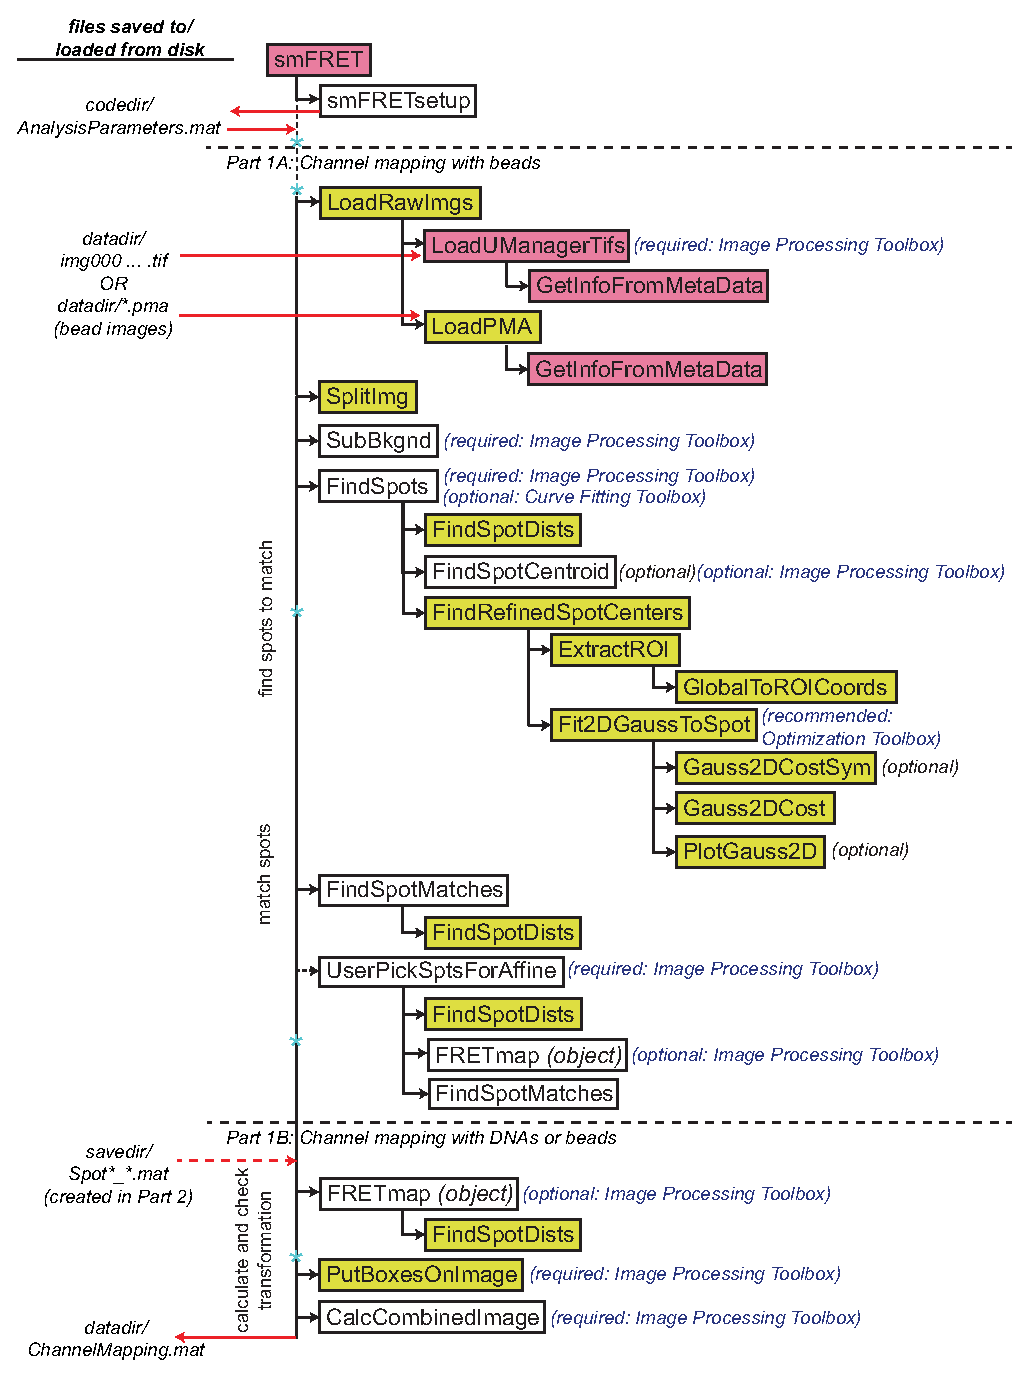
\includegraphics[width=6in]{CodeFlowchart.eps}
\caption{Call graph of the functions for calculating a channel mapping.}
\label{fig:CodeConnectivity1}
\end{center}
\end{figure}

\begin{figure}[!p]
\begin{center}
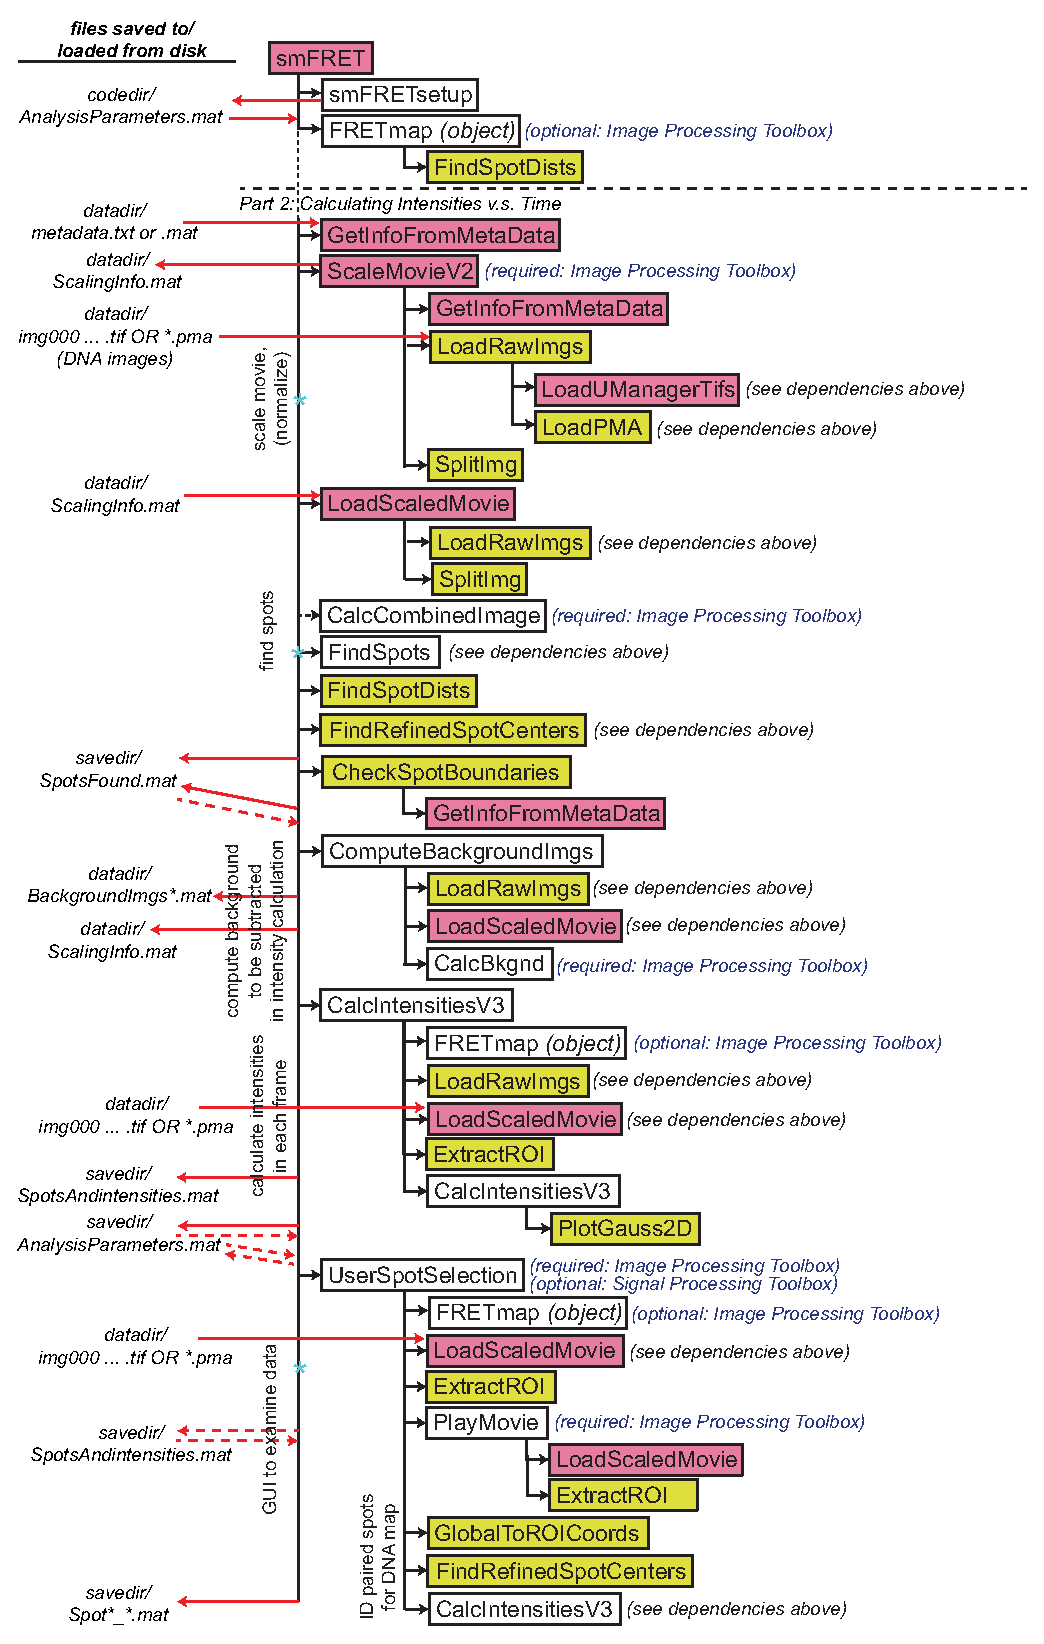
\includegraphics[width=5.4in]{CodeFlowchart2.eps}
\caption{Call graph of the functions for analyzing real data.}
\label{fig:CodeConnectivity2}
\end{center}
\end{figure}

\clearpage

\section{Running the analysis (and understanding what it does).}

Make the directory containing the smFRET analysis suite code your current directory, or add it to your current paths. Open the smFRETsetup.m file and change parameters as necessary. 

{\it For example, you will want to set } defaultdatadir, defaultsavedir, {\it and} codedir. {\it Follow the instructions under Display Defaults to make sure figures will show up well on your screen.  I recommend leaving most of the other parameters alone for now; most of them are explained below, and will make more sense once you've run the analysis once.}\\
\\
To start the analysis, enter\\

\noindent smFRET(`{\it rootname}')\\

\noindent in the command line (see Fig.~\ref{fig:DirectoryStructure} for a description of ``rootname'').  \\

%{\it For example, to analyze the data in my Sample FRET Data repository, the rootname would be \sj{``HighFRET10pM''}.} \\

\noindent Pass `1' as the second, optional input to run in debug mode, which will provide some additional figures (detailed below).\\

\noindent You will be asked (in the command line) if you want to create a channel mapping using beads (Part~1A), load an old one (Part~2), or create a channel mapping from paired DNAs saved in Part 2 below (Part~1B). 

{\it We (and others, e.g., \cite{Deindl2012}), routinely image a slide with surface-immobilized fluorescent beads to calculate at least a preliminary channel map.  This software does not support the creation of a map from real data} de~novo, {\it although there are workarounds that would allow it.  For example, you can load the FRETmap object (described below) included in this suite that contains the identity transformation instead of a calculated affine or polynomial transformation. Load this map using the ``L'' option, then use the GUI to generate paired spots that could be re-loaded using the ``D'' option.  However, without a bead-based map to get you close enough to see the real spot pairs in the GUI, your channels would have to be fairly well aligned to start with in order to make this work).}

%\sj{TODO: A potential bug I should figure out how to get rid of ... } 
{\it Note: any time it asks you to press ``anything else'', it will probably crash if you press the space bar. Choose a different anything else!  Also: If you're running in debug mode, and press ``enter'' to proceed when execution pauses, these ``enter'''s can get out of sync with the code being executed and may be counted as user input when you don't want them to be.  I suggest not using ``enter'' to proceed when Matlab indicates ``Paused: Press any key''.}

\subsection{Part 1A: Creating a channel map from fluorescent beads.}

(1) When prompted, navigate to the directory that contains the bead directories. \\

\noindent (2) If there is more than one directory with ``Bead'' in its title in the directory you choose, you will be given the option to use only some of the Bead data in creating a map, and to use the remaining bead data to quantify the fidelity of the mapping. 

{\it I usually collect data on 4-5 fields of view of our bead slide, use 2-3 of them to create a map, and use the remaining ``held-out'' data to check the transformation. }%See Sec.~\ref{sec:TformPracticals} for some advice, based on my experience, on how many beads you need per field of view to get a good transformation, how much the transformation varies from day to day on our setup,} etc.\\

\subsubsection{Spot finding.}\label{sec:SptFindBds}

{\it Spot finding is accomplished by finding local maxima and local minima across the image, and then calling real spots those maxima that are sufficiently larger than their local minima; the rest of the local maxima, that fall below the threshold, represent fluctuations in background.  This method has the advantage of not setting an absolute intensity threshold for real spots that must apply across the entire image, thereby allowing the illumination to vary across the image.  The Ha lab code does something roughly equivalent: they use a single absolute threshold value across the entire image, but they spot-find on a background-subtracted image. (In the Ha lab code, the threshold is hard-coded into} nxgn1\_cm {\it (spot finding for beads) and} p\_nxgn1\_ffp {\it and} ...\_brief {\it (spot finding for DNAs), in the parameter ``std''.) I prefer to keep spot-finding and background subtraction as separate procedures that can be modified independently without changes to one impacting the other.}\\

\noindent (3) Spot finding is done on one channel at a time, on an averaged image of the first FramesToAvg frames (where FramesToAvg is set in smFRETsetup; the Ha lab uses a hard-coded value of 10 frames). The spot-finding routine in FindSpots will attempt to identify an appropriate threshold value that distinguishes background fluctuations from real spots. The number of spots (``peaks'') that, according to this threshold, are considered to be real signal are printed to the command line. A further refinement of all peaks found is then performed; the basic refinement that is always performed excludes spots too close to the edges or to another spot (where ``too close'' is defined as closer than DNASize or BeadSize pixels in smFRETsetup). The smFRET wrapper function passes an input pair (``Method'', ``GaussFit'') that does an additional refinement by fitting a 2D Gaussian to each peak and insisting that the variance is not too small (which is usually the case when a very bright single pixel got included as a ``spot''), and the local background is not too high (which happens when two beads are right next to each other, but only one was found as a local maximum). The number of peaks kept after these refinements are then printed to the command line.

{\it I don't think the Ha lab code excludes peaks too close to one another---though it does exclude spots that aren't surrounded by sufficiently low intensity values at a radius of 5 pixels from the local maximum---so my code may find fewer spots per field of view than you're used to if you use the Ha lab code, though hopefully a higher percentage of the spots found will be useful, especially for real data.}\\

\begin{figure}
\begin{center}
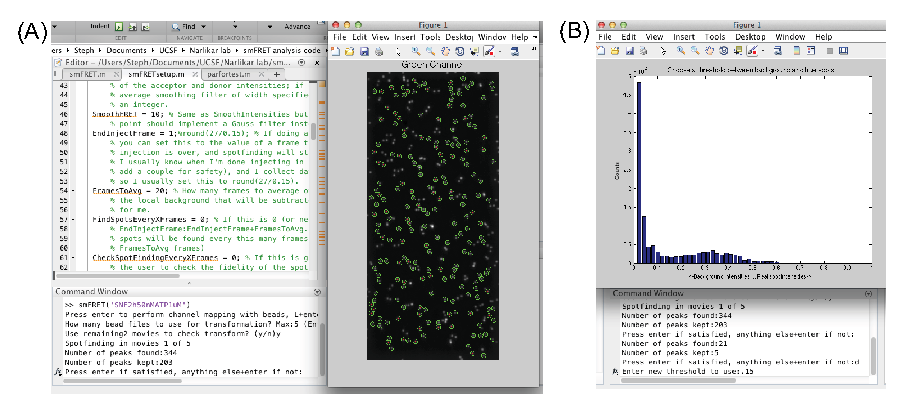
\includegraphics[width=6.5in]{ScreenShots/BeadFindScreenShot.eps}
\caption{Screen shots of the spot finding routine. These are for spot finding on beads, but would be similar with real data. (A) The figure on the righthand side of the screen shows the donor channel half of the image from the camera, with green circles around each spot identified as a bead. (B) If the automatic threshold detection fails (as it obviously did here), you can set the threshold manually, using as a guide a histogram of the difference between each local maximum and its local minimum.  With the beads it's easy to identify a good threshold---notice the two clearest peaks, one near zero that represents background, and one around 0.3 that represents the beads. The vertical dashed line indicates the current threshold value. }
\label{fig:BeadFindShot}
\end{center}
\end{figure}

\noindent (4) Examine the image displayed, with green circles around spots found, and the information displayed at the command line. Press enter to accept the results, anything else+enter to choose a new threshold.  A screenshot taken at this point in the analysis is shown in Fig.~\ref{fig:BeadFindShot}(A).\\

\noindent (5) If you rejected the results, a histogram of the differences between all local maxima and local minima will be displayed (as in Fig.~\ref{fig:BeadFindShot}(B)), with a vertical black line at the current threshold value.  For the beads, there should be two clear peaks in the histogram, one near 0 (which represents fluctuations in background), and one which on our setup peaks around 0.2-0.3 (and maybe some small bumps at higher values that represent double beads, extra bright junk on the slide, {\it etc}). (These peaks won't be so clearly distinguishable with single dyes, but the same principle will apply there too.) Choose a new threshold value and press enter.  Spot finding will be redone with this new threshold, after which you will again be given the option to accept the results or try another threshold.

{\it NOTE(1): you must enter a threshold value before pressing enter, even if you've changed your mind and want to keep what it used the last time!  The current threshold prints to the command line, if you want to re-enter it.}

{\it NOTE(2): The number of peaks found can be changed by changing the threshold (larger threshold will result in fewer peaks found); the number of peaks kept can be changed by changing the BeadSize parameter in smFRETsetup (or, for spot finding with real data, the DNASize parameter), and/or the cen\_tolerance and VarTolerance parameters at the beginning of FindRefinedSpotCenters.m, and/or the bkgnd\_tolerance parameter near the beginning of FindSpots.m.}  \\

\noindent (6) Continue spot-finding in the other channel, and repeat for all bead movies you are going to use to calculate the mapping and to check the mapping. 

{\it On our setup, the number of peaks found per field of view, with our bead slide, should be about 300-350, and with reasonable parameter settings the number of peaks kept should be about 175-200.}

\subsubsection{Spot pairing.}

\noindent (7) For every Bead directory examined, after spots have been found in each channel, the number of spots paired will be printed to the command line. 

{\it If your microscope's channel alignment is pretty good, the number of spots paired should be about 80\%-90\% of the spots found. The pairing code uses a ``greedy algorithm'' to match spots, which essentially means it assumes for each spot that its match in the other channel isn't too far away, and is probably the closest one.  Some mismatches at this point are ok; they will be removed before the final mapping is calculated (even a couple mis-pairings out of hundreds of true pairs can really mess up the fidelity of the mapping!).} \\

\noindent {\it If running in debug: after spots have been found in each channel, and before pairing is attempted, a figure will be displayed that shows the full image (both channels together) with white circles around each spot found.  Execution will be paused until the user presses a key.} \\

\begin{figure}
\begin{center}
\includegraphics[width=6.5in]{ScreenShots/SpotMatching}
\caption{Screen shots of the debugging figures for the spot-matching routine, and of the manual pairing option for poorly aligned channels. (A) If running in debug mode, after spots have been found in each channel and then paired, a figure of the full image from the camera (left) with green circles around the paired spots will be displayed, and a plot of matched points in each channel overlaid on each other, with a blue line connected them (right). These figures are for a fairly good alignment on our microscope. Note the shape of the ``vector field''---this gives a picture of the polynomial transformation that must be used to map between channels. Note also the mispairings---having only a couple mispairings, as here, is not a problem at this point; they will be removed before the final map is calculated, because they are obvious outliers.  More than a couple mispairings, however, and it will not be clear enough what are outliers and what are real pairs for a map to be generated. (B) Same as the left figure in (A) but for a particularly bad alignment of the emission side optics. (C) For poor alignments like in (B), a greedy pairing algorithm will not work, since the correct spot to pair is not necessarily the closest one.  In this case, the user will be shown a full image from the camera and will be asked to pick a spot in the red channel, then its pair in the green, then another spot in the red, until three pairs have been picked. (Specific instructions are printed to the command line.)  Spots are circled in white after they are selected.  White lines show the cross-hairs that Matlab displays for the user to pick points.}
\label{fig:PairingShot}
\end{center}
\end{figure}

\noindent (8) If your channels aren't aligned well on the microscope, however, it may not get enough correct matches to get a good enough transformation to pick out the mismatches.  In this case, the user will be asked to select three pairs of spots that are true matches (see Fig.~\ref{fig:PairingShot}(C)), from which an affine map will be calculated that will then be used to automatically match the rest of the spots.  It's best to choose three spots that span as much of the image as possible.  (By the way, if you're wondering, why 3?---Three is the minimum number of points necessary to define an affine transformation.  More details about affine transformations can be found in Sec.~\ref{sec:Details} below.)

{\it This is actually what the Ha lab code does from the start, essentially: it asks the user to identify three pairs of spots, creates a rough affine map to match more spots, and then uses those additional spots to generate a polynomial transformation (which requires a minimum of 15 spots, for the polynomial used in our code, or minimally 16 spots for the polynomial used in the Ha lab IDL code).  But, the more the better, because then you will have more information about the form the polynomial mapping takes for more of the field of view.}

{\it NOTE: If you have a lot of spots in the field of view and/or the mapping is pretty far off from the identity transformation, the matching algorithm may still fail even with a user-generated affine map to help it.  If that happens, you'll be asked to pick a different set of three pairs from which to create an affine map; if it still fails, the number of spots will be reduced (if you start with enough) a couple times in an attempt to get a good set of matches. (The problem with too many spots, if each spot is more than a couple pixels off from its pair in the other channel, is that the greedy algorithm, which picks the nearest spot as the best match, may have too many nearby spots to choose from.)}\\

\noindent {\it If running in debug: after spots have been paired, a new figure of the whole image will be displayed, this time with only the spots paired circled in green.  A second image that overlays the locations of the spots found in one channel on those found in the other, with a blue line connecting the ones it thinks are matches, will also be displayed, as shown in Fig.~\ref{fig:PairingShot}(A).  I've found this second figure to be useful to visualize the alignment of the emission side optics on the microscope.  Execution will again be paused until the user presses a button.}

\subsubsection{Calculating the transformation that maps from one channel to the other.}

{\it The mapping from one channel to another is accomplished by a mathematical transformation that relates a point in one channel to a point in the other channel.  A best-fit transformation is calculated from paired sets of points, one set in each channel.  As discussed in more detail below (see Sec.~\ref{sec:Details}), we and others have found a 4th-degree polynomial to best describe the relationship between channels.  The degree and kind of polynomial fitted, and the option to use affine instead of polynomial, are set in smFRETsetup.  Both IDL and Matlab have built-in functions to fit polynomial or affine transformations; the FRETPmap class object also includes hand-written code to do the same, though using Matlab's optimized (and professionally written) versions are always preferable when possible. (You will have to use my hand-written code if, for example, you want to fit a maximum degree 4 polynomial, which Matlab's built-in polynomial class does not support; see also Sec.~\ref{sec:Details}.)}\\

\begin{figure}
\begin{center}
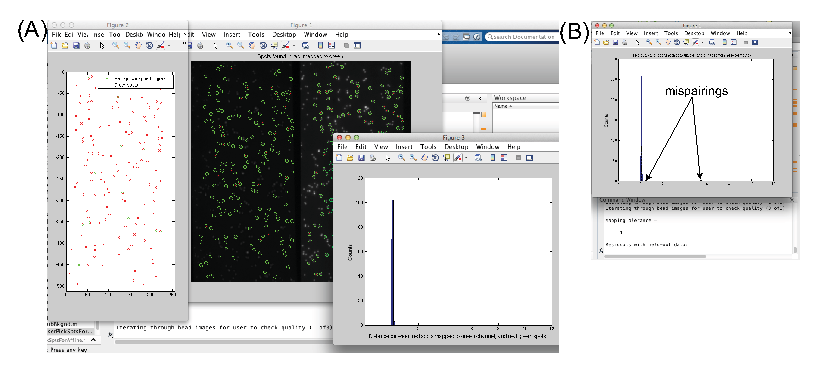
\includegraphics[width=6.5in]{ScreenShots/CheckMap.eps}
\caption{Screen shot of the figures that are displayed for the user to check the channel mapping. (A) For each Bead movie that was used to calculate the mapping, two sets of figures will be displayed, with a pause in between.  The first set contains 5 figures that allow the user to check the mapping fidelity from donor to acceptor channel, three of which are shown here: an image of the full view of the camera, with the spots used to calculate the mapping circled in green; a scatter plot of the locations of the centers of all the acceptor-channel spots, and of where the mapping thinks their centers should be; a histogram of the distances between the real acceptor-channel spots and where the mapping thinks they should be; and overlays of the donor channel onto the acceptor, using either an affine or a polynomial transformation (not shown).  (NOTE: if you have a version of Matlab older than 2013, which doesn't have Matlab's overlap function {\it imwarp}, you'll get a warning ``CalcCombinedImage: your version of Matlab does not support this function'', and you will have only three figures, not five.) While the histogram is generally the most useful of these figures, the scatter plot and image can be useful for picking out where the mapping is failing, if it is.  Note that there should be no counts above about 1 pixel in the histogram. The second set of figures is the same as the first three listed here, but for the inverse (acceptor to donor) transformation (the images shown here are actually for the inverse transformation). (B) If the user chose to keep some bead images as held-out data on which to check the transformation (that is, spot-find and pair in some images, but don't use this information to calculate the transformation), after the previous sets of figures have been displayed for all bead images used to calculate the transformation, a histogram will be displayed showing the distances between mapped acceptor spots and real acceptor spots.  In this case, there may be some residuals at higher pixel values, which should be mis-pairings in the held-out data. (I've found that if the residuals look fine for the data used to generate the map, it's not necessary to check the residuals for the inverse transformation as well, so only the residuals for donor-to-acceptor are displayed.) }
\label{fig:MapCheckShot}
\end{center}
\end{figure}

\noindent (9) After spots have been found and paired in all Bead directories, a preliminary mapping will be calculated, and then refined by the removal of obvious outliers, which are mis-paired or poorly localized spots.  After every cycle of refinement, the remaining number of spots that are being used to calculate the mapping, and the residuals for the current map, will be printed to the command line.  These residuals are the sum of the squared differences between mapped spot locations and real spot locations.  The refinement process will insist that the residuals per spot drop below the ResidTolerance value in smFRETsetup; if it can't manage that, it will halt in the debugger and print some instructions to the command line about how to proceed.

{\it Note that the residuals printed are summed over all spots; the ResidTolerance parameter is per spot, so a ``ResidualsGtoRperSpot'', which is the residuals divided by the total number of spots included in the transformation, is also printed to the command line, for comparison to the tolerance.  Note also that because we usually calculate a polynomial transformation, which is not invertible (unlike affine), a separate transformation is computed for acceptor to donor channel, and donor to acceptor; therefore both sets of residuals (``ResidualsGtoR'' and ``ResidualsRtoG'', where ``R'' stands for ``red'' and means ``acceptor'', and ``G'' means donor (``green'')) are printed.  There are also two sets of figures that display, one for one direction, one for the reverse.  They're generally pretty similar (both the figures and the residuals), but it's good to check both.}\\

\noindent (10) The final channel mapping will be saved (along with some additional information) in the same directory as the Bead files used to generate it. The map is contained in a FRETmap object.  A number of figures (see Fig.~\ref{fig:MapCheckShot}) are then displayed so that you can check how well the transformation did.  The most important of these are the histograms of distances between mapped spots and real spots. For the held-out data, if any (that is, bead data that wasn't used for the transformation), the vast majority of these distances should cluster between 0 and 0.5 pixels.  There will always be some counts in the histogram at higher values---these represent mis-pairings.  However, the mapping will only be useable if the difference between where it thinks a spot is and where it actually is, for true pairings, is less than about 0.5 pixels.  For the non-held-out data, there should be no mismatches, and the differences between real spots and mapped spots should be mostly below ~0.2 pixels.  Lastly it will print a Mapping Tolerance to the command line.  This is the maximum distance, rounded up to the nearest whole pixel, at which you can be confident a spot in one channel and a spot in the other are a pair.  For a good channel mapping on our setup, the Mapping Tolerance should be 1 for beads (2 for single dyes).

{\it NOTE (1): In order to (manually) load the FRETmap object back into Matlab, if you want to play around with it, you must have the directory containing the FRETmap.m class definition file in your known paths (or in your current directory).}

{\it NOTE (2): One of the sets of figures that are displayed at the end, if your version of Matlab is 2013 or later, includes overlays of one channel over the other, using either an affine transformation (which does better) or polynomial (which does worse, even though when comparing fit residuals the polynomial does significantly better).  This would be used to calculate a combined image, if you wanted to spot-find using a combined image to more easily catch mid-FRET spots.  For reasons that I'm still not clear on, it (very obviously) does not work with Matlab's built-in overlay functionality ... so for the moment, at least on our setup, using a combined image to find spots is not an option. I've not had a problem, however, finding mid-FRET spots, by changing the threshold in the spot-finding routine, and/or by spot-finding every 100 or so frames.}

\subsection{Part 2: Generate and examine FRET-versus-time traces.}

(1) After you've calculated a map, or if you chose to load an old one, navigate (when prompted) to the directory that has the data directory/directories you want to analyze, whose names should start with the ``rootname'' entered as the argument to smFRET.

\begin{figure}
\begin{center}
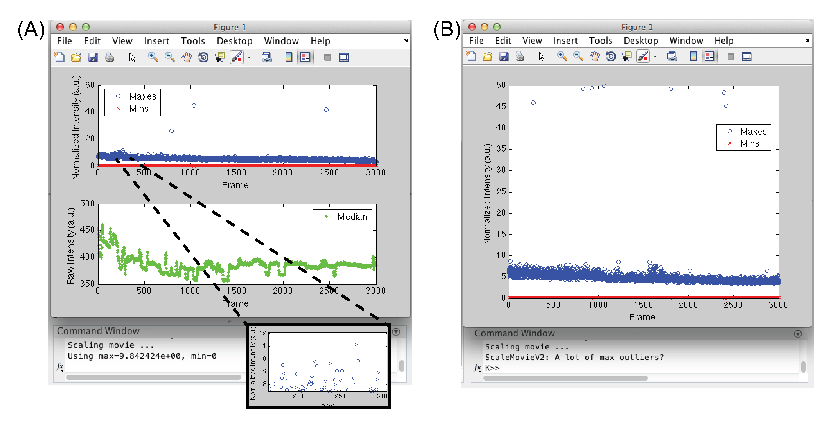
\includegraphics[width=6in]{ScreenShots/ScalingScreenShots.eps}
\caption{Screenshots for the movie scaling (data pre-processing) steps. (A) For every frame in a movie, the minimum (top panel, red), 99.99th percentile (top panel, blue) and median (bottom panel, green) intensity values are calculated and displayed.  The horizontal black line on the top panel indicates the max value to which all intensities will be scaled.  %The inset shows a zoom of the maxima around 250 frames, which includes the maximum that will be used for the scaling.  
The maximum and minimum values to be used for scaling are printed to the command line and execution is paused so that the user can confirm the values are reasonable. (Note that if ScaleChannelsSeparately is set to 1 in smFRETsetup, there will be an additional panel between the two shown here, that shows the 99.99th percentiles for the two channels separately, and the max and min to which each channel will be scaled will be printed to the command line.)  The bottom panel shows the roughly 7\% median intensity value fluctuations that we have observed with one of our lasers, which we believe are due to laser intensity fluctuations.  If these are not removed, these fluctuations will show up in all intensity-versus-time traces for individual spots and obscure real signal.  If the NormImage parameter in smFRETsetup is set to 1, each frame will be normalized to (specifically, divided by) its median value, removing the median intensity fluctuations.  (B) To choose a reasonable 99.99th percentile to use as the max, outliers in these percentiles are first removed. If more than 7 of them are removed, execution will pause and ask the user to confirm that the scaling algorithm is truly removing outliers or if it is starting to remove real maxima.  If the maxima plot looks like it does in (B), where there are more than 7 clear outliers, enter ``dbcont'' in the command line to override the checkpoint.  (You may have to do that several times, if there are more than 8 outliers in the maximum intensities and the scaling algorithm will pause after each one to check that it's still only removing outliers.)}
\label{fig:ScaleMovieShot}
\end{center}
\end{figure}

\subsubsection{Scaling and (optionally) normalizing images.}

{\it Scaling refers to taking the raw images from the camera, which are sometimes in a slightly weird numeric type (like uint14's), and whose actual intensity values don't span the full available range of that numeric type, and doing two things to them: converting to a more common numeric type (like uint8's, or doubles), and linearly expanding the actual image intensities to take advantage of the full dynamic range available.  Taking advantage of the full dynamic range available means telling Matlab what value to call ``white'' and what value to call ``black''---ideally you want your brightest pixels (those with the highest intensity values) to display as white, and the darkest (those with the lowest intensity values) to display as black.  Let's say your camera saves uint14 images; that means the available range of values each pixel can have is [0 16383].  Matlab, or any other program you use to display the raw images, will assume 16383 means white, and 0 means black.  Usually, however, most pixel intensity values will be much, much smaller than 16383, so everything will display as essentially black.}

{\it There are three reasons you'd want to scale images.  The first has to do only with presenting the data to the user in a helpful way, NOT with anything that actually affects the Cy3 and Cy5 intensity values, or FRET values, you get out of the data.  By scaling the raw intensity values to the full dynamic range, the user can see all the features of the image clearly when the image is displayed on the screen, because you tell Matlab to pick a more reasonable intensity value than the never-approached 16383 to call ``white''.  As long as you do a linear scaling, scaling to the available range does not change anything about the actual information you get out of the images, because each pixel's} relative {\it value to every other pixel remains the same.  The second reason you'd want to scale your images is related to the first, in that many of Matlab's built-in image processing toolbox functions want images scaled on the interval [0~1] (which is, for our purposes here, Matlab's preferred ``dynamic range'').  That is, Matlab wants the brightest intensity value, the one you want displayed as white, to have a value of 1, the lowest intensity value, which should display as black, to be zero, and everything else scaled between 0 and 1. Many of Matlab's functions also want to be given doubles, not uint14's or uint8's; the built-in Matlab function that scales a given image or set of images to [0~1],} mat2gray, {\it also converts to double precision.  Finally, depending on your setup, it may be necessary to scale the donor and acceptor images to different maxima---meaning, the value that gets set to ``white'' for acceptor may not be the same as for donor images---so that acceptor and donor intensities can be directly compared (discussed more below).  Unlike scaling the entire (donor+acceptor together) images to a maximum that makes displaying the image nice, scaling the donor and acceptor images separately will, obviously, change your results (most importantly, your calculated FRET values).}

{\it Choosing the maximum value to which all intensities should be scaled can be nontrivial. The Ha lab acquisition code scales to minimum and maximum intensity values set (with some user oversight) before acquisition begins.  The UCSF mrc to pma converter scales to the minimum and maximum intensity values across the entire movie.  This can be somewhat sub-optimal, because there are often a few very, very bright pixels (outliers in the distribution of intensities, often caused by ``dirt'' on the slide or similar) that will get set to white and everything that you care about set to nearly black.  Since the UCSF mrc to pma converter is only used to make our data compatible with the Ha lab IDL code, which doesn't display images for the user to inspect anyway, the maximum the converter chooses doesn't really matter.  However, since this smFRET suite does frequently display images for the user, I have found that a better way to scale each movie is to use an intensity value that represents the 99.99th percentile of all the intensities in the movie.\footnote{Technically, ScaleMovie calculates the 99.99th percentile from each frame, and then takes the max value of those percentiles.  It works out to be about the same, and doesn't much matter anyway.}  It's very important to make sure that no real data intensities get set to 1, the highest possible value, so that you don't ``cap'' real information in your image, which is why the 99.99th percentile is chosen (that should be well above the actual intensities of any real data, well out into the tail of very-bright-dirt outliers in the intensity distribution).}

{\it More importantly for our setup, though, is the option of scaling the donor and acceptor images to different maxima.  In smFRETsetup you can set whether to scale the donor and acceptor channels separately, using the ScaleChannelsSeparately parameter.  Possibly because of some of the filters in our microscope setup, our donor channel is always slightly dimmer than the Cy5 channel; therefore we scale the donor images to the 99.99th percentile value that the donor side takes on, and the acceptor images to the 99.99th percentile value that the acceptor side takes on.  This essentially puts the donor and acceptor intensities reported for each spot in the GUI on the same set of axes, so that they can be directly compared to one another.  }

{\it You can tell that a movie is appropriately scaled by two metrics: first, that the acceptor and donor spots are easy to see in the images that display with the GUI (see below); and second, that the maximum acceptor and donor intensities in every trace are roughly equal.  That is, if you have a FRET-ing molecule, and the acceptor bleaches, the donor should rise to the same value as the acceptor (unless you have reason to believe that shouldn't be the case for your system).}

{\it Finally, we've had problems with laser intensity fluctuations; therefore if NormImage is set to 1 in smFRETsetup, all pixels in each frame will be normalized to the median intensity value in each frame to remove these fluctuations.} \\

\noindent (2) ScaleMovie will display the ``maximum'' (99.99th percentile), minimum and median intensity values for the movie as a function of frame, and print the values it's going to set to 0 (min across the movie) and 1 (max across the movie) to the command line (see Fig.~\ref{fig:ScaleMovieShot}(A)).  Then it will pause and wait for you to press any button to accept and proceed.  If it has to remove a lot of outliers to find a good maximum to scale to, it will stop in the debugger and ask for user input.  If everything looks fine anyway, enter ``dbcont'' into the command line to proceed.

\subsubsection{Spot finding.}

\noindent (3) Spotfinding proceeds as described for the beads in Sec.~\ref{sec:SptFindBds} above, with the option of the following modifications that are controlled by parameters in smFRETsetup:

(a) If instead of only finding spots in an averaged image of the first FramesToAvg frames, you want to find spots throughout the movie, set the FindSpotsEveryXFrames parameter to a value greater than 0.  After an initial round of asking the user to set a good threshold for real spots, spot finding will proceed with this same threshold until a multiple of CheckSpotFindingEveryXFrames (see next point) is reached.

(b) I highly recommend setting the CheckSpotFindingEveryXFrames parameter to a value equal to FindSpotsEveryXFrames or to 5*FindSpotsEveryXFrames, or something like that.  At least with my data, the optimal threshold varies enough over, say, 100 frames that if you just keep using the threshold for the first FramesToAvg frames, you run the risk of a significant number of false positives (background fluctuations that get counted as real spots) or missing real spots because the threshold was too high or too low.  Working on improving the automatic threshold detection ... {\it NOTE: If you're running in debug mode, every CheckSpotFindingEveryXFrames, it will display a figure showing the new spots that have been found since the last round, in red, and all old spots in green, for each channel. }\\

\noindent (4) At the end of the spot finding session, all spots found in both channels will be saved to the directory you chose to save data in ({\it savedir}).  In addition, a list of spots in the frame of reference of the acceptor channel will also be saved, as follows: spots found in the donor channel are converted to the frame of reference of the acceptor channel, using the channel map that you just calculated or that you loaded, and if a donor spot was found close by to an acceptor spot ({\it e.g.}, if that spot was a mid-FRET spot and so showed up in both channels), the location of the spot in the acceptor channel will be saved---so that you don't double-count spots.  This final list of spots in the frame of reference of the acceptor channel will be saved as the ``spots'' variable in the SpotsFound.mat file saved to {\it savedir}, and it is this list that will be used to calculate intensities for each spot.

{\it NOTE (1): Any time after this point, you can quit out of smFRET, rerun smFRET with the same input argument ({\it i.e.} the same rootname), load a different channel map, and then load the spots found in both channels and re-convert to the acceptor channel frame of reference, by selecting the ``Load previously found spots?'' option (NOT the ``Load previously found spots and their intensities?'' option).  Spot intensities will then be re-calculated. (Since spot-finding is independent of a channel map and happens for each channel separately, you don't have to find spots again just because you want to change where their pair in the other channel should be.  There are also options to re-scale the movie without re-finding spots.  See more details in Sec.~\ref{sec:AnalysisOptions}.)}

{\it NOTE (2): If you load the SpotsFound.mat file you will also notice that variables called} Vars, VarsR {\it and} VarsG {\it are saved.  These contain the $x$- and $y$-variances of the best-fit 2-D Gaussian used to refine each spot's location.}  VarsR {\it and} VarsG {\it are the variances for spots found in the acceptor channel (saved to the} RefinedCentersR {\it variable) and in the donor channel (}RefinedCentersG{\it) respectively. } Vars {\it has the same length as} spots {\it and contains the variances that will be used in the intensity calculation.  For any spot found in only one channel, that spot's variances is used; however if a spot was found in both channels, the variance of the spot in the acceptor channel is saved.  These variances are used if the IntensityGaussWeight parameter in smFRETsetup is 1 and FixSpotVar is the empty matrix.}

\subsubsection{Calculating the background.}\label{sec:BkgndSub}

{\it At this point a background image is calculated for each frame and saved to disk, for use in the next step in calculating the intensity of a spot.  A visual inspection of TIRFM images will demonstrate that the background is not constant over the entire field of view (to a greater or lesser extent depending on the shape of the TIRF spot relative to the field of view, among other things).  Moreover, we know that every image will consist of a lot of background, with some very localized real signal (that is, spots that represent fluorescence from the dyes).  Our background estimation routine first smooths the images, to smooth out contributions from the punctate real data, and then median-filters\footnote{CalcBgknd actually uses the built-in Matlab function imopen, which is much faster than the options for doing a median filter and results in almost the same thing.} the image to pick out the slowly spatially-varying background (and then smooths this calculated background a little more).  This background calculation procedure is essentially the same as the Ha lab's, except we calculate one background image for every frame instead of one for the whole movie from an average of the first 10 frames, allowing for a time-varying background due to laser intensity fluctuations or other factors.}

{\it NOTE: This is currently the longest step of analysis---on my laptop this takes $\sim$5-7 minutes for a data set with $\sim$3000 frames.  Therefore this step is done only right before you need it---so that you can find spots and examine the quality of the movie in the previous step before investing the time to calculate the background.  Note also that because these background images are saved as double precision, for best compatibility with Matlab's toolboxes, and there's one for every frame of your movie, they're going to take up a relatively large amount of additional disk space---for example, as much as 4x the original movie size, if the original movie was saved in int16 precision like ours are.  You can delete these files after you've completed the next step (calculating intensities vs time), but they will be re-generated every time you analyze a particular data set. }

\subsubsection{Calculating intensities-per-time for each spot.}

{\it Nominally, calculating the intensity of a spot in each frame is simple---the intensity is just the sum of the intensities of all the pixels defined as part of the spot. However, there are several refinements that are usually done before this sum is calculated: (1) A background value is subtracted before the intensities are summed.  Ideally, after a fluorophore has bleached, the summed intensity should drop to approximately zero, if the background was effectively subtracted. (2) A weighted average instead of a straight average is performed by some groups (including the Ha lab). If the IntensityWeightGauss option is 1 in smFRETsetup, which I highly recommend, each spot's intensity will be weighted, in each frame, with a 2D gaussian centered on the spot and having the amplitude you set in GaussWeightAmp. This has the effect of smoothing out some of the fluctuations in a spot's intensity due to noise. The Ha lab uses an amplitude of 2, which just stretches the results out along the intensity axis.  Also, you can either weight with a Gaussian whose width is fixed to the values set in FixSpotVar; or you can weight each spot by a Gaussian whose width was calculated when the spot was originally found. The Ha lab fixes the spot variances; I've found it doesn't make a huge difference. Using spot-specific variances can be nice if part of the field of view has distortions that result in more ellipsoid, rather than round, spots.  (Note that if you want ellipsoid spots, the UseSymGauss option must be 0.)}\\

\noindent (5) Raw (that is, unsmoothed, if smFRETsetup has smoothing options selected) intensities for donor and acceptor channels will be calculated and the results will be saved to the save directory, as a ``SpotsAndIntensities'' file.  Note that at this point, FRET values are not calculated, nor are any corrections to the intensities (like alpha) or modifications like smoothing, so any relevant options in smFRETsetup (alpha, gamma, SmoothFRET and SmoothIntensities) can be changed by changing smFRETsetup and rerunning.

{\it Any time after this point, you can quit out of smFRET and re-load traces into the GUI, without recalculating their raw intensities, by selecting the ``Load previously found spots and their intensities?'' option.  Use this option if, for example, you want to change the smoothing values in smFRETsetup and then rerun the GUI.  You will be asked if you want to load the GUI with old parameters; if you've changed smFRETsetup, select ``n''.}

\subsubsection{The GUI.}\label{sec:GUI}

\noindent (6) A GUI will appear with a figure showing intensity-versus-time and FRET-versus-time traces, and a separate figure showing (initially) an average of the first FramesToAvg frames. Note that the displayed intensities and FRET values are smoothed and have the correction factors gamma and alpha applied (see smFRETsetup for definitions of gamma and alpha); that is, they are NOT the raw intensities (though these raw intensities are saved along with modified intensities---see below). Instructions for GUI options print to the command line. Most options should be straightforward, with the possible exceptions of:

``b'' (background adjustment): If the background subtraction routine didn't remove all the background ({\it i.e.}, intensity values are significantly nonzero after photobleaching), select this option, then click on two parts of the intensity-versus-time or FRET-versus-time trace over which you want to define a new background value. The average donor and acceptor intensities between these two points will be subtracted from every point. 

``r'' (reset background): remove any additional background subtraction you added with the ``b'' option.

``z'' (zoom): Click on two points in the intensity-versus-time or FRET-versus-time traces to zoom in on that area.

``u'' (unzoom): undo any zoom. NOTE that this will define how much of each trace is saved---see below.

``f'' (show a particular frame), ``m'' (play movie between two time points), ``a'' (show average around a particular frame): In the case of ``f'' or ``a'', click on a point in the intensity-versus-time or FRET-versus-time traces that you want displayed in Fig. 1.  Note that if you go forward or backwards a spot, Fig. 1 will reset to an average of the first FramesToAvg frames.  ``m'' will leave Fig. 1 showing the last frame loaded (but again Fig. 1 will reset if you go forwards or backwards).

``l'' (re-Locate spot): If the channel mapping didn't find a spot pair well in one channel, you can click on where you think the true spot center is, and smFRET will attempt to re-find the spot in that area, and then re-calculate the intensities using that new spot center. (This may take a few minutes.)  Note: if a new spot center is successfully found, this new center, and the newly calculated intensities, will be saved to the ``SpotsAndIntensities'' file.  If you want to revert to original spot locations, you'll need to re-load from the ``Load previously found spots?'' point. \\

{\it NOTE: You don't need to press enter after making a selection---for example, to go forward one spot, just press ``.'', no enter needed.  Any time you enter something into the command line, however, you do need to press enter---for example, if you select ``g'' to go to a particular spot, you will be prompted to enter the spot number in the command line, after which you } will {\it need to press enter.  You need to make all selections with Fig. 2 current---if you don't, you'll notice you'll just type stuff into the command line and nothing will happen ... }\\

\noindent (7) What is saved to disk when you select the ``s''  option in the GUI: When you select ``s'' for a spot, a new file will be created in the save directory called ``Spot$<$movienum$>$\_$<$spotnum$>$.mat'' (or if you select ``s'' for a spot for which a file has already been created, you will overwrite the previous file with a new one).  This file contains: 

(a) vectors of raw donor and acceptor channel intensities for each FRAME (``rawRedI'', ``rawGrI''); 

(b) vectors of unsmoothed, but with alpha applied for the acceptor intensities and gamma applied for FRET values, donor and acceptor intensities and FRET values for each frame (``unsmoothedRedI'', ``unsmoothedGrI'', ``unsmoothedFRET'')---NOTE it is these intensities and FRET values that are used in ConvertTovbFRETInput, which converts all saved ``Spot*\_*.mat'' files in a directory into a single input file that can be loaded into vbFRET \cite{Bronson2009};

(c) vectors of donor and acceptor intensities and FRET values with any smoothing applied (``RedI'', ``GrI'', ``FRET'')---these will be identical to the unsmoothed versions if no smoothing was applied;

(d) The frame rate at which data were acquired (``fps'', which is actually frames per MILLISECOND)

(e) The ($x,y$) coordinates of the center of the spot in the donor channel and the acceptor channel, in the coordinate systems of their respective channels (note these coordinates will depend on the value of PxlsToExclude in smFRETsetup) (``Rspot'',``Gspot''), and the variance used for the Gaussian weighted sum, which is assumed to be the same for both channels (``variance'').

In addition to this Spot file, an eps and a Matlab .fig file of whatever is in Fig. 2 will also be saved, with the same filename.  NOTE: Only what is in Fig. 2 will be saved---meaning if you zoomed in on part of the trace, the Spot file will only contain the intensities and FRET values for the zoomed region.  You can choose to cut out parts of traces this way (for example, you can choose not to keep everything after both fluorophores have bleached).  If, however, you decide you want to restore part of the trace you cut, just re-load this data set into the GUI and use the ``u'' command to un-zoom---the full raw intensities are still saved in the ``SpotsAndIntensities.mat'' file.

\subsection{Part 1B: Creating a channel map from paired DNAs.}

You can make a map using true paired DNAs (that you've confirmed are true FRET pairs by their intensity traces, and that you made sure, using the GUI, were well-localized) by running smFRET with any input,  selecting the ``D'' option, and navigating to a save directory that contains the ``Spot$<$$>$.mat'' files saved with the ``s'' option from the GUI.  As with the beads, a transformation will be calculated, the residuals refined as much as possible, and then the user will be asked to check the results.  Works the same as described above for beads, although most of the figures that are generated for bead maps will not be generated here.   NOTE: You need at least 15 pairs of spots in order to calculate a polynomial transformation (at least of degree 4, as we and others usually do); if Matlab spits out a bunch of warnings about poorly conditioned fits, and/or you have close to or fewer than 15 spots, try changing to ``MatlabAffine'' in smFRETsetup.

\subsection{Summary of analysis options.}\label{sec:AnalysisOptions}

\noindent{\it After making or loading a map, for every movie you will be asked:}\\

\noindent $\Rightarrow$ {\it If a ``SpotsAndIntensities.mat'' file exists from a previous analysis:} ``Load previously found spots and their intensities? (y/n)''  \\

$\Rightarrow$ {\it If you select ``y'':} ``Use old parameters? (y/n)'', and go straight to GUI.\\

$\Rightarrow$ {\it If you select ``n'' and a ``SpotsFound.mat'' file exists:} ``Load previously found spots? (y/n)''  \\

\indent\indent $\Rightarrow$ {\it If you select ``y'' (use old spots):} ``Use same channel mapping as last time but recompute: 
\indent\indent\indent scaling, background, intensities? (y/n)''\\

\indent\indent\indent {\it If you select ``y'' (use old mapping):} The same spots as were displayed in the GUI last
\indent\indent\indent\indent  time will be kept (including their numbering), but the movie will be re-scaled, and new
\indent\indent\indent\indent background images and intensities for each spot will be computed.\\

\indent\indent\indent {\it If you select ``n'':} Spots found in the two channels will be loaded, and a new list of spots 
\indent\indent\indent\indent will be generated based on whatever channel mapping you loaded at the start.  Use  
\indent\indent\indent\indent this option if you don't want to re-find spots but do want to change the mapping you  
\indent\indent\indent\indent used to associate a red spot with a green spot.  HOWEVER: note that this will change 
\indent\indent\indent\indent the numbering (and likely the total number) of the spots found, so any spots you found 
\indent\indent\indent\indent before will not have the same indices as the last time you ran the GUI.  Spot intensities 
\indent\indent\indent\indent are recalculated, but not background images.\\

\indent\indent $\Rightarrow$ {\it If you select ``n'' and a ScalingInfo.mat file exists:} ``Load scaled movie? (y/n)''\\

\indent\indent\indent\indent {\it If you select ``n'', the movie is re-scaled, then new spots are found, background subtraction 
\indent\indent\indent\indent\indent information created, and spot intensities re-calculated.}\\

\indent\indent\indent\indent {\it If you select ``y'', the movie is re-scaled and background is NOT recalculated, but new
\indent\indent\indent\indent\indent spots are found and their intensities calculated.}\\

\noindent {\it Note: To re-calculate the background without re-scaling, delete the ``BackgroundImgs*.mat'' files in} savedir.

\newpage

%\section{Customization Options.}\label{sec:CustomOpts}
%
%\noindent \textbullet~FindSpots:
%
%\noindent \textbullet~CalcBkgnd and SubBkgnd:
%
%\newpage

\section{Details and derivations.}\label{sec:Details}

\subsection{Channel mapping/transformations: General concepts}\label{sec:TransformGeneral}

The essence of finding a map that relates locations in the donor channel to locations in the acceptor channel, and vice versa, is finding a transformation in the mathematical sense.  We will be particularly concerned with massaging the desired channel maps into \textit{linear} transformations, because linear transformations can be described by matrices, and we can bring the power of linear algebra to bear on them.  In particular, for a set of points (think spots---beads or dyes---in one of the channels) $\vec{x} = \{\vec{x_1},\vec{x_2},...,\vec{x_n}\}$, where the Cartesian coordinates of each point are given by $\vec{x_i} = (x_{i1},x_{i2})$, we can write a linear transformation to the other channel in terms of a matrix {\bf A}, such that 
\begin{equation}
\vec{y} = \mathbf{A}\vec{x}, \label{eqn:SimpleMap}
\end{equation}
where $\vec{y}$ are the Cartesian coordinates of the points in the other channel.  We will use the same convention for $\vec{x}$ and $\vec{y}$ as in the code, namely, that a single spot's coordinates will be a column vector, and so a set of spots will be a 2x$n$ matrix, where $n$ is the number of spots.  Then we know that in the simple example of Eqn.~\eqref{eqn:SimpleMap} above, {\bf A} will be a 2x2 matrix, though this will not be the case for all of the transformations we describe below.  

The goal, of course, is to find {\bf A}, which will be the map describing how to find a spot's location in the other channel, if we know where it is in the first channel. More precisely, what we want is a {\it best fit} value for {\bf A}. That is, we want to find the {\bf A} that minimizes the error of our estimate of $\vec{y}$, given $\vec{x}$; {\it i.e.} we want to find {\bf A$^*$} such that
\begin{equation}
\mathbf{A^*} = \underset{\mathbf{A}}{\textrm{argmin}}\Vert {\vec y} - \mathbf{A}\vec{x}\Vert_2^2. \label{eqn:findbestA}
\end{equation}
According to Eqn.~\eqref{eqn:findbestA}, {\bf A$^*$} will be the {\bf A} that minimizes the difference between the true positions of the points represented by $\vec{y}$, and where we estimate them to be based on applying matrix {\bf A} to $\vec{x}$. (The notation $\Vert ... \Vert_2$ just means the ``norm-2'' (Euclidean norm or Euclidean distance) of whatever is between the $\Vert$'s; in 2-space, you will recall that for two points $(x_1,x_2)$ and $(y_1,y_2)$, their Euclidean distance is $\sqrt{(x_1-y_1)^2+(x_2-y_2)^2}$.) 

How do we find {\bf A$^*$}? We use the {\bf normal equations} as conditions of optimality. 
%The normal equations state that $\vec{y} - \mathbf{A^*}\vec{x}$ need to be orthogonal to the rowspace of $\vec{x}$ \textcolor{red}{(err ... or the rowspace of Ax?)}, in order for {\bf A$^*$} to fulfill Eqn.~\eqref{eqn:findbestA}. By the definition of orthogonality, this means that
I refer you to a linear algebra textbook that discusses the normal equations for more details, but, in short, using the normal equations as conditions for optimality means we want to find {\bf A$^*$} such that
\begin{equation}
(\vec{y}-\mathbf{A^*}\vec{x})\cdot\vec{x}^T = \vec{0}. \label{eqn:NormalEquations}
\end{equation}
%If it's been a while since you've thought about rowspaces and the like, here's another, more intuitive way to think about Eqn.~\ref{eqn:NormalEquations}: The rowspace of $\vec{x}$ is the plane? surface? described by treating each row of $\vec{x}$ as a point in 3-space. \textcolor{red}{(Um ... given my points are 2xn, should I be talking about the columnspace of x ... ? Getting stuck here, Matt, help!!)}
(If you want some intuition about what's going on here, think about reading Eqn.~\ref{eqn:NormalEquations} row-wise: The first row is an orthogonality statement that constrains the first row of {\bf A}, saying that the first row of the residual, that is, the stuff in the parenthesis on the left-hand side, should be orthogonal to the row space of $\vec{x}$. The second row of Eqn.~\ref{eqn:NormalEquations} says that the second row of the residual should {\it also} be orthogonal to the row space of $\vec{x}$---meaning we have two orthogonality constraints that must be satisfied on {\bf A$^*$}.)

Now what we need to do is solve Eqn.~\eqref{eqn:NormalEquations} for {\bf A$^*$}. Rearranging Eqn.~\eqref{eqn:NormalEquations} and moving the term containing {\bf A$^*$} to the other side, we have
\begin{equation}
\vec{y}\vec{x}^T = \mathbf{A^*}\vec{x}\vec{x}^T.
\end{equation}
Remember these are matrices, so we cannot ``divide'' both sides by $\vec{x}\vec{x}^T$, but we can multiply both sides of the equation, on the righthand side, by the inverse of $\vec{x}\vec{x}^T$. Is $\vec{x}\vec{x}^T$ invertible? You can show that it is (which I'm not going to do here, but you can Wikipedia linear least squares and/or look up the normal equations in a linear algebra textbook if you'd like to know more).  So we have our final solution that 
\begin{equation}
\vec{y}\vec{x}^T(\vec{x}\vec{x}^T)^{-1} = \mathbf{A^*}. \label{eqn:NormEqnsSolution}
\end{equation}

{\bf In summary}, to find the best-fit transformation that takes a set of spots $\vec{x}$ in one channel to a set of spots $\vec{y}$ in another channel, we calculate the lefthand side of Eqn.~\ref{eqn:NormEqnsSolution}. In practice, Matlab has a smarter way of solving these equations, represented by the slash operator. So in the channel mapping code of this repository, you will find {\bf A$^*$} computed as $\vec{y}\vec{x}^T/(\vec{x}\vec{x}^T)$ rather than as written in Eqn.~\ref{eqn:NormEqnsSolution}.

\subsection{Affine versus polynomial maps.}

Before we describe how to find {\bf A}, or more precisely, how to fit it using a set of control points whose locations we know in both channels, we first give some intuition about what the different transformations implemented in this code do to a set of spots.  

\subsubsection{Affine transformations.}

\begin{figure}
\begin{center}
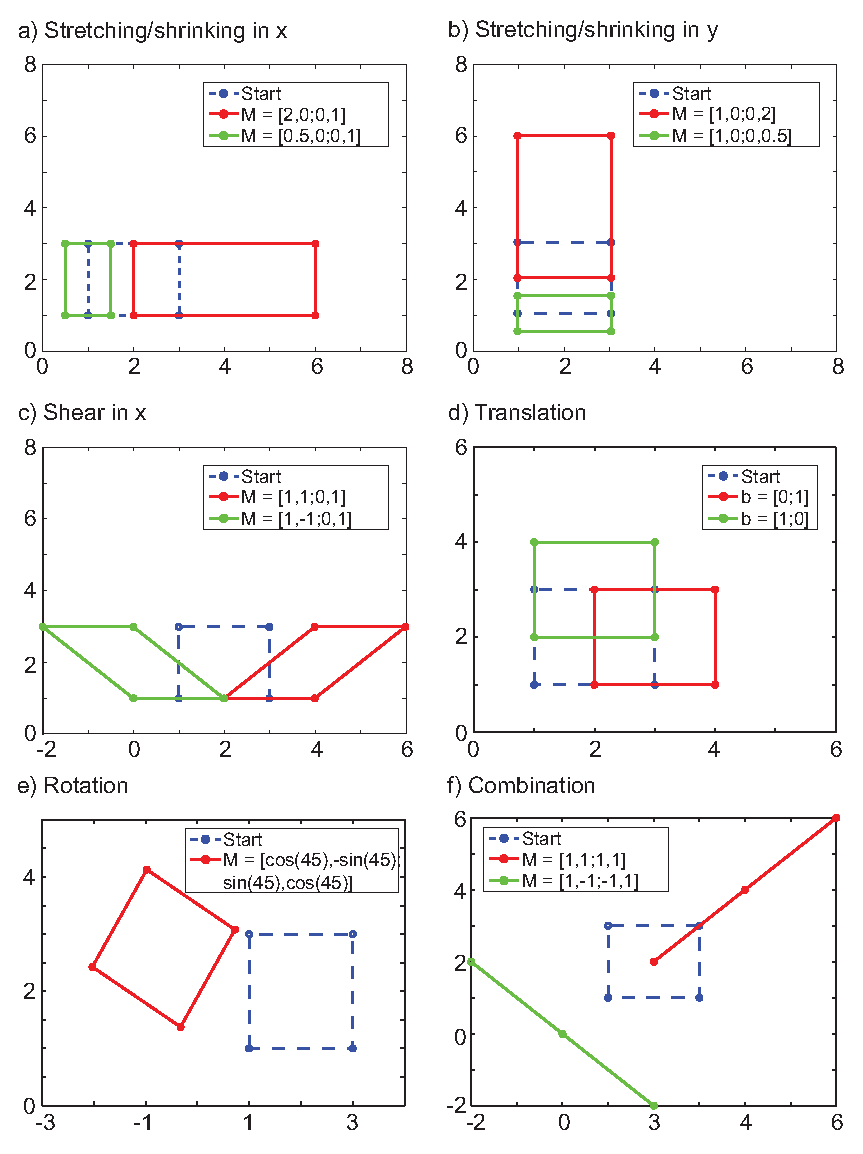
\includegraphics[width=5in]{TransformationFigures/AffineExamples.eps}
\caption[Examples of affine transformations.]{{\bf Examples of affine transformations.} In all panels, the blue box outlined in dashed lines represents $\vec{x}$, the starting set of points. The legends show the choice of {\bf M} or $\vec{b}$ that gives the transformed set of points $\vec{y}$, shown in green or red.  Where not listed, {\bf M} = [1, 0; 0, 1]; and $\vec{b}$ = [0,0]. }\label{fig:AffineExamples}
\end{center}
\end{figure}


Affine transformations allow for stretching/shrinking, rotation, shear, translation, and reflection (which isn't really applicable to TIRF microscopy).  An affine transformation can be represented as 
\begin{equation}
\vec{y} = \mathbf{M}\vec{x} + \vec{b}\label{eqn:affine}
\end{equation}
Fig.~\ref{fig:AffineExamples} shows how the elements of {\bf M} and $\vec{b}$ accomplish the various changes possible with affine maps.  As we will see below, an affine transformation describes donor-acceptor pairs of spots in smFRET fairly well, though a polynomial transformation tends to do slightly better (in our hands as well as in others'---see, for example, \cite{Joo2007,Deindl2012}).\footnote{We note here that the Ha lab IDL code first generates an affine map, by asking the user to pick three true pairs of spots (three being the minimum number of points needed to define an affine transformation), and uses this to automatically match more spots with which to generate a polynomial map.}

\subsubsection{Polynomial transformations.}

Polynomial transformations represent a more general and less well-defined class of transformations than affine transformations, and in fact, as we will see, even the terms used to describe them in the IDL versus Matlab documentation differ in significant ways.  

A polynomial transformation is one in which each element of the output vector, $y_{j1}$ and $y_{j2}$, is determined by a polynomial of the input vector elements, $x_{i1}$ and $x_{i2}$.  The polynomials for $y_{j1}$ and $y_{j2}$ can be different. An example of a very simple polynomial transformation is 
%\begin{equation}
%       \left[   \begin{matrix} 
%          y_1 \\
%          y_2
%          \end{matrix} \right] = \left[ \begin{matrix}
%          			3+x_1+2x_2\\
%				 1+5x_1+ 3x_2
%				 \end{matrix} \right]
%\end{equation}
\begin{align}
      y_1 &=  3+x_1+2x_2\\\notag
      y_2 &= 1+5x_1+ 3x_2
\end{align}
Each term (3, $x_1$, $2x_2$, {\it etc}) is called a {\bf monomial}.  Note that this is actually a linear system of equations, and therefore is in fact an affine transformation---it can be written in matrix form as in Eqn.~\eqref{eqn:affine} above.  This means that polynomial transformations can do to a set of points all of the things shown in Fig.~\ref{fig:AffineExamples}, as well as other things.

To be a polynomial transformation that is not affine, the {\bf degree} of one or both of the polynomials that define the transformation must be greater than 1. Degree is defined in two ways: the {\bf maximum degree} is the highest power of a single variable that appears in the polynomial; for example, in the polynomial $3+x_1x_2+x_1^2x_2$, the maximum degree is 2.  The {\bf total degree} is the highest power of combinations of variables that appears; for example, in the polynomial $3+x_1x_2+x_1^2x_2$, the total degree is 3.

This distinction becomes important when we look at the polynomial transformations that can be fit to sets of control points using IDL's POLYWARP function versus Matlab's fitgeotrans function.  IDL defines the degree of the polynomial to be fit as the {\it maximum degree}, whereas Matlab defines the degree of the polynomial to be fit as the {\it total degree}.  The Ha lab IDL code uses POLYWARP to fit a ``third-degree'' polynomial to control points to find the channel mapping; Matlab's fitgeotrans only implements total degree 2, 3, or 4 polynomials, which means we cannot use Matlab's built-in functionality to fit the same kind of polynomial as in the Ha lab code.  To be specific, POLYWARP with a degree 3 polynomial allows terms like $x_1^3x_1^2$, because the maximum degree for that polynomial is 3; but because its total degree is 5, this monomial would not be included in a degree-4 polynomial fit (or a degree-3 fit) by Matlab's fitgeotrans.

We will examine below how these different polynomial transformations affect a set of points, but first we specifically define polynomial transformations according to IDL's POLYWARP and Matlab's fitgeotrans.  POLYWARP finds parameter vectors $\vec{K_x}$, $\vec{K_y}$ such that, for a starting set of points $\left[\begin{smallmatrix} x_1\\ x_2\end{smallmatrix} \right]$ and an ending set of points $\left[\begin{smallmatrix} y_1\\ y_2\end{smallmatrix} \right]$,
\begin{equation}
       \left[   \begin{matrix} 
          y_1 \\
          y_2
          \end{matrix} \right] = \left[ \begin{matrix}
          			\sum_{i,j=0}^D K_{x_{i,j}} x_1^ix_2^j\\
				\sum_{i,j=0}^D K_{y_{i,j}} x_1^ix_2^j
				 \end{matrix} \right], \label{eqn:POLYWARPdef}
\end{equation}
where $D$ is the degree of the polynomial fit (set by the user). Note that for a maximum degree of 3, the highest-order term possible here is total degree 6, namely $x_1^3x_2^3$.  More explicitly, we can write out Eqn.~\eqref{eqn:POLYWARPdef} as 
\begin{align}
y_1 &= K_{x_{00}} + K_{x_{10}}x_1+K_{x_{01}}x_2+K_{x_{11}}x_1x_2+K_{x_{20}}x_1^2+...\\
y_2 &= K_{y_{00}} + K_{y_{10}}x_1+K_{y_{01}}x_2+K_{y_{11}}x_1x_2+K_{y_{20}}x_1^2+...
\end{align}
Although POLYWARP returns $\vec{K_x},\vec{K_y}$ as vectors, we can think of them as matrices, with the rows corresponding to the coefficients for each monomial in $x_1$ ($x^0$(=constant),$x$,$x^2,...$) and the columns corresponding to the coefficients of each monomial in $x_2$.  That is, for a degree 3 polynomial fit, we can arrange the elements of $\vec{K_x}$ as
\begin{equation}
 \begin{matrix} 
            & \mathbf{x_2^0}         & \mathbf{x_2^1} & \mathbf{x_2^2}  & \mathbf{x_2^3} \\
\mathbf{x_1^0} & K_{x_{00}} & K_{x_{01}} & K_{x_{02}} & K_{x_{03}} \\
\mathbf{x_1^1} & K_{x_{10}} & K_{x_{11}} & K_{x_{12}} & K_{x_{13}} \\
\mathbf{x_1^2} & K_{x_{20}} & K_{x_{21}} & K_{x_{22}} & K_{x_{23}} \\
\mathbf{x_1^3} & K_{x_{30}} & K_{x_{31}} & K_{x_{32}} & K_{x_{33}}
\end{matrix} 
\end{equation}
and similarly for $\vec{K_y}$.  Note that there will therefore be 32 coefficients (16 for $K_x$, 16 for $K_y$) for a degree 3 polynomial fit in IDL.

On the other hand, Matlab's documentation (see images.geotrans.PolynomialTransformation2D class) tells us that a degree 2 polynomial fit returns a $\vec{K_x}$ vector of length 6 for a 2-degree fit, length 10 for degree 3, and length 15 for degree 4.  This means that a third degree fit in Matlab will have only 20 parameters, rather than the 32 of IDL.  Even the degree 4 fit will have only 30 parameters; though this will result in a fit of a comparable number of parameters to the IDL degree-3 fit, the particular monomials that are allowed in that fit will be different.  In particular, a third-degree fit in Matlab will return a $\vec{K_x}$ vector that would correspond to the matrix
\begin{equation}
 \begin{matrix} 
            & \mathbf{x_2^0}         & \mathbf{x_2^1} & \mathbf{x_2^2}  & \mathbf{x_2^3} \\
\mathbf{x_1^0} & K_{x_{00}} & K_{x_{01}} & K_{x_{02}} & K_{x_{03}} \\
\mathbf{x_1^1} & K_{x_{10}} & K_{x_{11}} & K_{x_{12}} & - \\
\mathbf{x_1^2} & K_{x_{20}} & K_{x_{21}} & - & - \\
\mathbf{x_1^3} & K_{x_{30}} & - & - & -
\end{matrix} 
\end{equation}
where we have indicated monomials that are not included in the fit by a dash.

How much does the degree of the polynomial, and the allowed monomials, affect the goodness of fit for pairs of smFRET spots?  Is it simply the number of parameters that is important---do we just need ~30 parameters to capture all the degrees of freedom of the microscope image---or the kinds of monomials that matter most?  This question is addressed in Sec.~\ref{sec:AffineVsPoly} below.

\subsection{Finding non-linear transformations.}

In Sec.~\ref{sec:TransformGeneral} we described how to find the best-fit {\it linear} transformation, given a set of control points whose positions we knew with reasonable accuracy in both channels. Comparing Eqns.~\eqref{eqn:NormalEquations} and~\eqref{eqn:affine}, it is not immediately obvious how to use the normal equations to find an affine transformation, and it is even less clear how to find a polynomial transformation.

What we need to do is to embed the affine and polynomial transformations in a linear space, such that they take the form of Eqn.~\eqref{eqn:SimpleMap}. It is actually relatively straightforward to do this for an affine transformation. Redefine $\vec{x}$, $\vec{y}$, {\bf M}, and $\vec{b}$ as $\vec{x}^\prime$, $\vec{y}^\prime$, and {\bf A} such that 
\begin{equation}
\vec{x}^\prime = \left[ \begin{matrix} \vec{x} \\ 1 \end{matrix} \right],
\end{equation}
\begin{equation}
\vec{y}^\prime = \left[ \begin{matrix} \vec{y} \\ 1 \end{matrix} \right],
\end{equation}
and
\begin{equation}
\mathbf{A} = \left[ \begin{matrix} \mathbf{M} & \vec{b} \\
							0 & 1 \end{matrix} \right].
\end{equation}
(All we're doing is adding a row of one's to $\vec{x}$ and $\vec{y}$, and combining {\bf M} and $\vec{b}$ into a new matrix along with a new row of two 0's and one 1.  Note that for an affine transformation in 2-space, {\bf M} is 2x2 and $\vec{b}$ is 2x1---see also Fig.~\ref{fig:AffineExamples}.) It should be clear that now $\vec{y}^\prime = \mathbf{A}\vec{x}^\prime$ is a linear transformation, whose solution for a best-fit {\bf A} is given in Eqn.~\eqref{eqn:NormEqnsSolution}, and that it is equivalent to the affine transformation of Eqn.~\eqref{eqn:affine}.\footnote{Note that Matlab's built-in affine transformation calculation function (cp2tform or fitgeotrans, depending on your version of Matlab) uses a different convention than I use here. Matlab computes the transformation: transpose($\vec{y}^\prime$) = transpose($\vec{x}^\prime$){\bf A}$_{\textrm{Matlab}}$, such that {\bf A} = transpose({\bf A}$_{\textrm{Matlab}}^{-1}$), where {\bf A} is the transformation matrix in my notation.}  (If that second point is not immediately clear, do the matrix multiplication for {\bf A}$\vec{x}^\prime$ and see that the first row of the resulting matrix is $\mathbf{M}\vec{x}+\vec{b}$.)

We can do a similar thing to embed a polynomial transformation in a linear space, with some slight modifications. Instead of the redefinitions above, we will instead define a new variable $\vec{\widetilde{x}}$ such that 
\begin{equation}
\vec{\widetilde{x}} = \left[\begin{matrix} 1 \\
							   x_1\\
							   x_2\\
							   x_1x_2 \\
							   x_1^2\\
							    ... \end{matrix} \right],
\end{equation}
up to/including as many monomials as we want to include in our transformation, and where as a reminder $(x_1,x_2)$ are the Cartesian coordinates of each point in the starting vector $\vec{x}$.  Note then that if our transformation included, say, 20 monomials, and we have $n$ points in $\vec{x}$, $\vec{\widetilde{x}}$ would be a 20x$n$ matrix.  We define a new variable $\vec{\widetilde{y}}$ similarly. Then our transformation matrix $\mathbf{\widetilde{A}}$ will contain the coefficients of the polynomials that relate the elements of the input vector ($x_1,x_2$) to those of the output vector ($y_1,y_2$). 

Take, for example, the polynomial transformation 
\begin{align}\label{eqn:PolyEx}
      y_1 &=  3+x_1+2x_1x_2+4x_2^2\\\notag
      y_2 &= 1+5x_1x_2+ 3x_1x_2^2 
\end{align}
We would then have 
\begin{equation}
\vec{\widetilde{x}} = \left[\begin{matrix} 1 \\
							   x_1\\
							   x_1x_2\\
							   x_2^2\\
							   x_1x_2^2\end{matrix} \right] \label{eqn:PolyEmbedEx1}
\end{equation}
and
\begin{equation}
\mathbf{\widetilde{A}} = \left[ \begin{matrix} 3 & 1 & 2 & 4 & 0\\
						1 & 0 & 5 & 0 & 3 \end{matrix} \right]. \label{eqn:PolyEmbedEx2}
\end{equation}
As with the embedding of the affine transformation in a linear space above, it should be clear from Eqns.~\eqref{eqn:PolyEmbedEx1} and~\eqref{eqn:PolyEmbedEx2} that $\vec{\widetilde{y}} = \mathbf{\widetilde{A}}\vec{\widetilde{x}}$ is linear, and that $\mathbf{\widetilde{A}}\vec{\widetilde{x}}$ represents the polynomial transformation given by Eqn.~\eqref{eqn:PolyEx} above.  

Finally we note that in the case of polynomial transformations, the transformation must be explicitly calculated in both directions (acceptor to donor and donor to acceptor), whereas affine transformations are invertible and the transformation in both directions can be calculated, if the transformation is known for one direction.

%\subsubsection{Calculating the inverse transformation.}
%
%In the preceding sections we have focused on the question of finding a transformation that maps the points in one channel, denoted by $\vec{x}$, to the other channel, denoted $\vec{y}$. However, for smFRET we need to be able to go both directions. Here we take up the question of how to calculate the transformation from $\vec{y}$ to $\vec{x}$.
%
%For affine transformations this is straightforward: given an affine transformation $\vec{y} = \mathbf{M}\vec{x}+\vec{b}$, the inverse mapping is simply (according to the rules of linear algebra) $\vec{x} = \mathbf{M}^{-1}(\vec{y}-\vec{b})$.  This will work as long as {\bf M} is invertible, which we know to be the case because \textcolor{red}{... well at the very least it's square ... }
%
%For polynomial transformations, on the other hand, we cannot say that $\vec{\widetilde{x}} = \mathbf{\widetilde{A}}^{-1}\vec{\widetilde{y}}$; at the very least, it is unlikely that $\mathbf{\widetilde{A}}$ will be square. In this case, \textcolor{red}{we have to calculate the reverse transformation explicitly?}

\subsection{Channel mapping: Practical considerations.}\label{sec:TformPracticals}

This section considers several questions relating to the practice of creating and using channel mappings. Obviously these are most likely highly system specific.  However the most important practical consideration for generating an accurate mapping is more universal, and that is to get correctly matched red- and green-channel spot pairs.  The Ha lab IDL code does this by asking the user to hand-pick three pairs, which are then used to generate an affine mapping, which is good enough to find the spot-pair matchings that are then used to calculate a polynomial transformation.  The code described here instead uses a greedy algorithm (described above) to find spot pairs, calculates a polynomial transformation with them, and then excludes spot-pairs that were not well-fit by the calculated transformation and recalculates a new polynomial transformation.  In my experience the excluded pairs are always mismatches that shouldn't have been included in the transformation calculation anyway.  It is important to note, however, that even a handful of mismatches ({\it e.g.} 5-10 mismatched pairs out of almost 1000 pairs total) significantly reduce the accuracy of the calculated transformation.

All of the transformations mentioned in this section, unless otherwise noted, are total degree 4 polynomial transformations calculated using Matlab's built-in fitgeotrans functionality.

\subsubsection{Comparing affine and polynomial transformations of smFRET data.}\label{sec:AffineVsPoly}

%\sj{Going to have two figures in this section: one of a grid to which we apply various transformations, and the other of real channel data under affine vs. various polynomial transformations.}
%
%\sj{Sum of squared residuals for: Affine = 42.5; Poly,Max3 = 1.45; Poly,Tot3 = 1.62; Poly,Tot4 = 1.39 <- for 200 beads.}
%\sj{For a different mapping: Affine = 162; Poly,Max3=5, Poly,Tot3 = 5.7,Poly,Tot4 = 4.9 <-for 900 beads}
%
%We conclude that: (1) The complexities of the distortions between channels require more than the motions allowed by an affine transformation; therefore a polynomial transformation is required. (2) Since a polynomial transformation of total degree 4, with 30 parameters, does slightly better than a polynomial transformation of maximum degree 3 (and total degree 6), with 32 parameters, we conclude that it is not simply the addition of more parameters that improves a polynomial fit, but rather the increase in the complexity of the transformation by the addition of higher-order terms ($x^4$ rather than just $x^3$). Moreover, allowing additional cross-terms (for example, $x_1^3x_2^2$) also does not seem to improve the ability of the polynomial transformation to fit the channel mapping points, which may be why Matlab's built-in polynomial transformation function, which is part of the image processing toolbox, focuses on total degree not maximum degree.

{\it (not done yet)}

\subsubsection{How many spots are needed for a good mapping?}

%Consider a set of four bead movies of different areas on a bead slide, taken without removing the prism or the sample.  When the first movie, with about 170 beads, is used to calculate the transformation, and this transformation is used to estimate the locations of the beads in the other three movies (total of about 600 beads), it is able to do so to within half a pixel or less.  When instead the first two movies are used to calculate the transformation (about 350 beads total), that transformation estimates the locations of the beads in the other two movies to within 0.3 pixels or fewer.  When the first movie's beads are subsampled and used to calculated polynomial transformations, these transformations are able to estimate the locations of beads in the other movies to within about 1 pixel or less, even with as few as 50 beads selected out of the first movie's 170 beads.
%
%In conclusion, then, only one movie's worth of spots (100-200 spots) should be sufficient in order to calculate a good transformation, and indeed the Ha lab IDL code accepts only one movie with which to perform the mapping.  However, in the interest of good scientific paranoia I usually take 2-3 movies, to ensure at least one will have a good distribution of beads with which to calculate the transformation, and usually use all of the movies to calculate the transformation, to ensure that I get a good estimate of the channel mapping in all areas of the field of view. I also sometimes check the transformation I calculate on a given day by using 2 or 3 movies to calculate a transformation, and check how well it can find the beads in the other movie(s) (and this functionality is built into this analysis suite).

This question has a fairly simple answer: you need at least 3 points to define an affine transformation, and you need at least 16 points to define a max degree 3 polynomial in IDL (15 for a total degree 4 polynomial in Matlab).  Beyond that, you want enough points to sample the whole field of view, or at least you want your 3 (or 15 or 16) points to be well-spread across the field of view to calculate the mapping across the whole field of view.  In practice, I've found that $\sim$50 well-dispersed spots represents a good sampling of our 512-pixels-by-512-pixels camera's field of view. (But as noted above where the channel mapping procedure for beads is discussed, in the interest of healthy scientific paranoia, I shoot for 100-200 spots in each of 2-3 fields of view, and a couple additional fields of view to check the transformation.  This usually isn't feasible with real dyes, however---and as noted below, I've found the mapping to be different for dyes vs the beads I use.  In the case of single dyes, I try to get at least 50 FRET pairs in a field of view.)

\subsubsection{How much does the mapping vary over time?}

In theory, since the mapping between channels should depend only on the microscope's emission-side optics, the mapping should change only if those optics are adjusted by a user.  In practice, I have found that the mapping drifts a little over time, though not noticeably over the course of a day.  Consider, for example, two maps made two weeks apart.  (In this case I am considering maps made from paired FRET-ing dyes, not beads, though my experience is the results would be similar for beads.)  The average squared residual per spot, when one map is used on the other map's control point data, is about 0.9-1 pixel---that is, a map from two weeks before can find a spot's true location to within a pixel on average.  (Using the ``TformResiduals'' method of the FRETmap class to plot all of the distances between mapped and true spot locations shows that a spot's true location is off by no more than 1.5 pixels, when a two-week-old map is used.)  If you're weighting each spot's intensity by a Gaussian, that Gaussian needs to be off in the true center of the spot by no more than about a pixel.  So, it's probably good to make a new map each time you take data, or at least make a new map every week or so and check that the optics haven't drifted too much.

\subsubsection{Does the transformation differ significantly if it's calculated from beads versus real DNAs?}

Yes ... {\it not done yet}

\newpage

\section{Acknowledgements.}

This project was a collaborative effort with Matt Johnson and Luke Breuer, who made significant intellectual and time contributions to its development.  Although they were both involved in every stage of this suite's development, in particular the derivations in Sec.~\ref{sec:Details} were contributed by Matt, and the concepts for most of the figures that allow visualization of the analysis process (and the idea of being able to play the data movie next to the trace) were contributed by Luke.  I am also indebted to TJ Ha's lab at UIUC, which has made what I consider to be ``industry-standard'' smFRET code freely available on their website. In this repository I make frequent allusions to the Ha lab code, noting where my code differs from theirs and where I have followed their lead. Thanks to the UCSF SMUG crew (Margaret Elvekrog, Thomas Noriega, Megan Mayerle, Sarah Ledoux, Daniel Elnatan), the Narlikar lab, especially John Leonard, and Kai-Chun Chang at the National Taiwan University for helpful discussions about code as well as experimental development, and to Megan Mayerle for the DNAs used to create the sample data.  Financial support through NIH grants to my PI, Dr. Geeta Narlikar, and a Leukemia and Lymphoma Society Career Development program fellowship are gratefully acknowledged.

\bibliography{smFRETCodeBiblio}

\end{document}
